\section{Methods}

\section{Experiments}

% No Max-Pooling

\begin{figure}[htbp]
	\centering
	\begin{minipage}{0.8\textwidth}
		\centering
		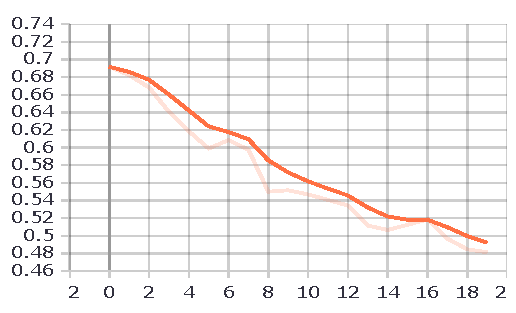
\includegraphics[width=0.6\textwidth]{Sources/Results/no_pooling/plots_pdf/epoch_TRAIN_D_mixed_loss.pdf}
		\subcaption[first caption.]{Training loss of the discriminator on mixed data, i.e. real and generated segmentation maps.}\label{fig:1a}
	\end{minipage}%

	\begin{minipage}{0.8\textwidth}
		\centering
		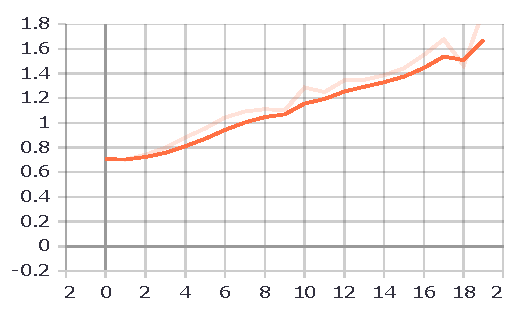
\includegraphics[width=0.6\textwidth]{Sources/Results/no_pooling/plots_pdf/epoch_TRAIN_GAN_from_D.pdf}
		\subcaption[second caption.]{Training loss of the generator, which is contributed by the discriminator.}\label{fig:1b}
	\end{minipage}%

	\begin{minipage}{0.8\textwidth}
		\centering
		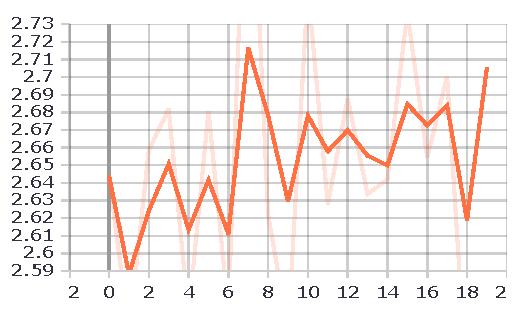
\includegraphics[width=0.6\textwidth]{Sources/Results/no_pooling/plots_pdf/epoch_TRAIN_GAN_from_G.pdf}
		\subcaption[third caption.]{Training loss of the generator caused by the reconstruction error, i.e. the dissimilarity between true and generated segmentation map.}\label{fig:1c}
	\end{minipage}

	\begin{minipage}{0.8\textwidth}
	\centering
	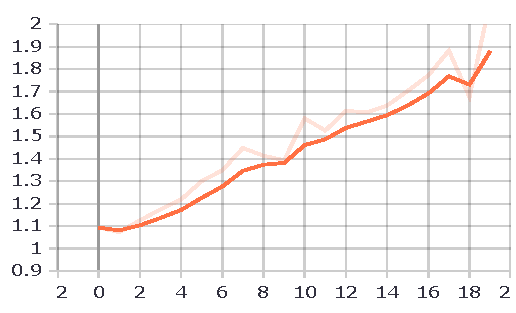
\includegraphics[width=0.6\textwidth]{Sources/Results/no_pooling/plots_pdf/epoch_loss.pdf}
	\subcaption[fourth caption.]{Total training loss of the generator.}\label{fig:1d}
	\end{minipage}
	
	\caption{Loss of the discriminator and generator during training.} \label{fig:1}
\end{figure}

\begin{figure}[htbp]
	\centering
	\begin{minipage}{0.8\textwidth}
		\centering
		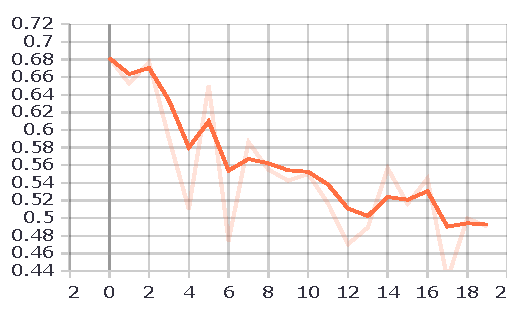
\includegraphics[width=0.75\textwidth]{Sources/Results/no_pooling/plots_pdf/epoch_VALIDATION_D_fake_loss.pdf}
		\subcaption[first caption.]{Validation loss of the discriminator on generated segmentation maps.}\label{fig:2a}
	\end{minipage}%
	
	\begin{minipage}{0.8\textwidth}
		\centering
		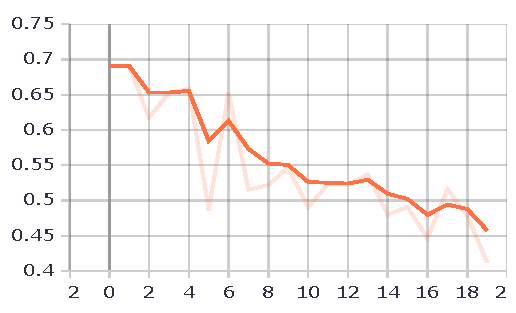
\includegraphics[width=0.75\textwidth]{Sources/Results/no_pooling/plots_pdf/epoch_VALIDATION_D_real_loss.pdf}
		\subcaption[second caption.]{Validation loss of the discriminator on real segmentation maps.}\label{fig:2b}
	\end{minipage}%

	\begin{minipage}{0.8\textwidth}
	\centering
	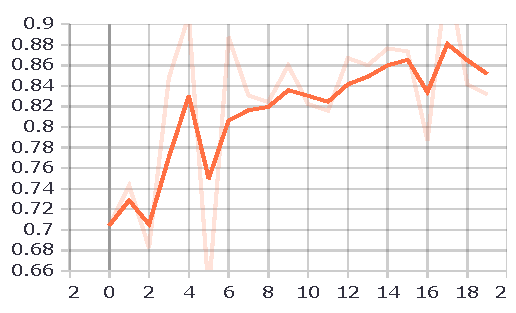
\includegraphics[width=0.75\textwidth]{Sources/Results/no_pooling/plots_pdf/epoch_VALIDATION_D_fake_acc.pdf}
	\subcaption[second caption.]{Validation accuracy of the discriminator on generated segmentation maps.}\label{fig:2c}
	\end{minipage}%
	
	\caption{Evaluation of the discriminator on validation data (with a batch size of $10$).} \label{fig:2}
\end{figure}

\begin{figure}[b]
	\centering
	\begin{subfigure}{.5\textwidth}
		\centering
		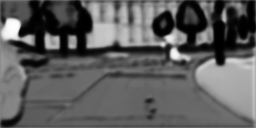
\includegraphics{Sources/Results/no_pooling/novelty_maps/novelty_map_1.png}
	\end{subfigure}%
	\begin{subfigure}{.5\textwidth}
		\centering
		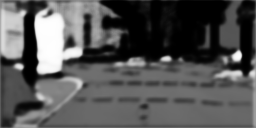
\includegraphics{Sources/Results/no_pooling/novelty_maps/novelty_map_2.png}
	\end{subfigure}
	\begin{subfigure}{.5\textwidth}
		\centering
		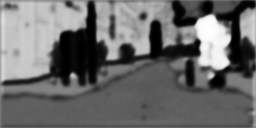
\includegraphics{Sources/Results/no_pooling/novelty_maps/novelty_map_3.png}
	\end{subfigure}%
	\begin{subfigure}{.5\textwidth}
		\centering
		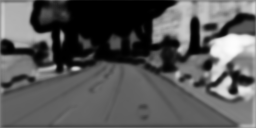
\includegraphics{Sources/Results/no_pooling/novelty_maps/novelty_map_4.png}
	\end{subfigure}
	\begin{subfigure}{.5\textwidth}
		\raggedleft
		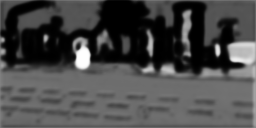
\includegraphics{Sources/Results/no_pooling/novelty_maps/novelty_map_5.png}
	\end{subfigure}
	\caption[short]{Some sample outputs of the GAN for different images with potential OOD objects.} \label{fig:novelty_maps_no_pooling}
\end{figure}

% Max-Pooling

\begin{figure}[htbp]
	\centering
	\begin{minipage}{0.8\textwidth}
		\centering
		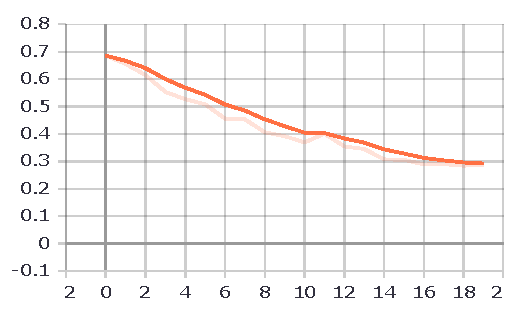
\includegraphics[width=0.6\textwidth]{Sources/Results/pooling/plots_pdf/epoch_TRAIN_D_mixed_loss.pdf}
		\subcaption[first caption.]{Training loss of the discriminator on mixed data, i.e. real and generated segmentation maps.}\label{fig:3a}
	\end{minipage}%
	
	\begin{minipage}{0.8\textwidth}
		\centering
		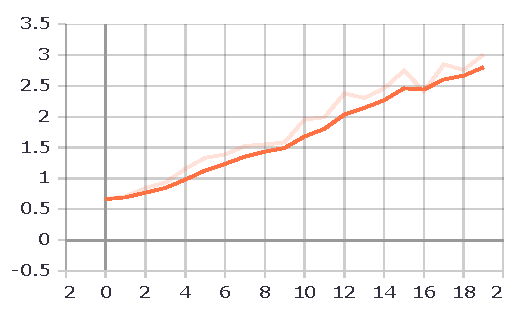
\includegraphics[width=0.6\textwidth]{Sources/Results/pooling/plots_pdf/epoch_TRAIN_GAN_from_D.pdf}
		\subcaption[second caption.]{Training loss of the generator, which is contributed by the discriminator.}\label{fig:3b}
	\end{minipage}%
	
	\begin{minipage}{0.8\textwidth}
		\centering
		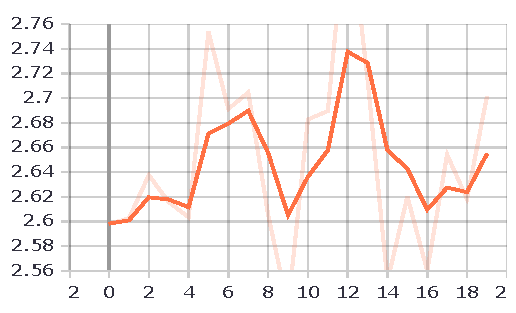
\includegraphics[width=0.6\textwidth]{Sources/Results/pooling/plots_pdf/epoch_TRAIN_GAN_from_G.pdf}
		\subcaption[third caption.]{Training loss of the generator caused by the reconstruction error, i.e. the dissimilarity between true and generated segmentation map.}\label{fig:3c}
	\end{minipage}
	
	\begin{minipage}{0.8\textwidth}
		\centering
		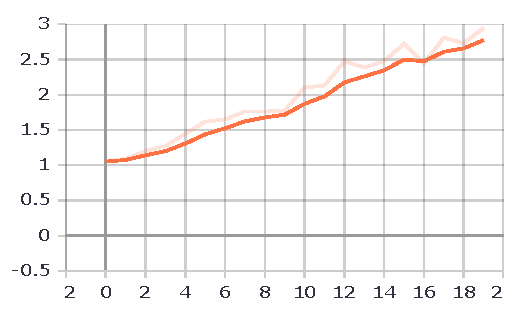
\includegraphics[width=0.6\textwidth]{Sources/Results/pooling/plots_pdf/epoch_loss.pdf}
		\subcaption[fourth caption.]{Total training loss of the generator.}\label{fig:3d}
	\end{minipage}
	
	\caption{Loss of discriminator and generator during training with additional max pooling in the discriminator.} \label{fig:3}
\end{figure}

\begin{figure}[htbp]
	\centering
	\begin{minipage}{0.8\textwidth}
		\centering
		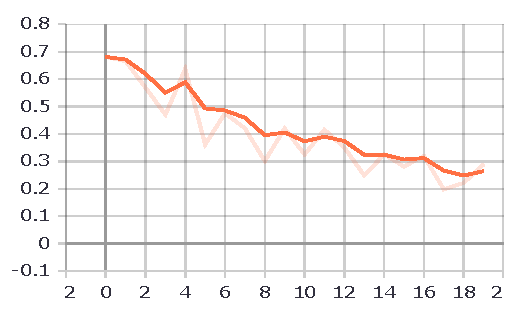
\includegraphics[width=0.75\textwidth]{Sources/Results/pooling/plots_pdf/epoch_VALIDATION_D_fake_loss.pdf}
		\subcaption[first caption.]{Validation loss of the discriminator on generated segmentation maps.}\label{fig:4a}
	\end{minipage}%
	
	\begin{minipage}{0.8\textwidth}
		\centering
		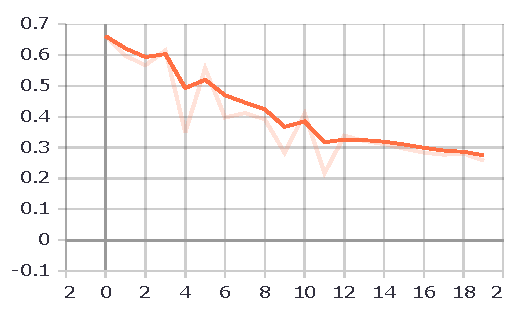
\includegraphics[width=0.75\textwidth]{Sources/Results/pooling/plots_pdf/epoch_VALIDATION_D_real_loss.pdf}
		\subcaption[second caption.]{Validation loss of the discriminator on real segmentation maps.}\label{fig:4b}
	\end{minipage}%
	
	\begin{minipage}{0.8\textwidth}
		\centering
		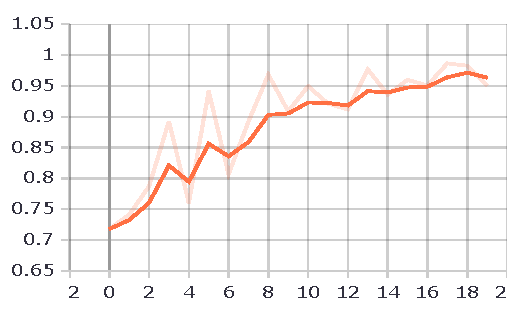
\includegraphics[width=0.75\textwidth]{Sources/Results/pooling/plots_pdf/epoch_VALIDATION_D_fake_acc.pdf}
		\subcaption[second caption.]{Validation accuracy of the discriminator on generated segmentation maps.}\label{fig:4c}
	\end{minipage}%
	
	\caption{Evaluation of the discriminator on validation data (with a batch size of $10$) using additional max-pooling in the discriminator.} \label{fig:4}
\end{figure}

\begin{figure}[b]
	\centering
	\begin{subfigure}{.5\textwidth}
		\centering
		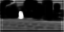
\includegraphics[width=1\textwidth]{Sources/Results/pooling/novelty_maps/novelty_map_1.png}
	\end{subfigure}%
	\begin{subfigure}{.5\textwidth}
		\centering
		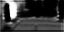
\includegraphics[width=1\textwidth]{Sources/Results/pooling/novelty_maps/novelty_map_2.png}
	\end{subfigure}
	\begin{subfigure}{.5\textwidth}
		\centering
		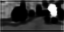
\includegraphics[width=1\textwidth]{Sources/Results/pooling/novelty_maps/novelty_map_3.png}
	\end{subfigure}%
	\begin{subfigure}{.5\textwidth}
		\centering
		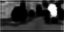
\includegraphics[width=1\textwidth]{Sources/Results/pooling/novelty_maps/novelty_map_4.png}
	\end{subfigure}
	\begin{subfigure}{.5\textwidth}
		\raggedleft
		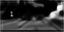
\includegraphics[width=1\textwidth]{Sources/Results/pooling/novelty_maps/novelty_map_5.png}
	\end{subfigure}
	\caption[short]{Some sample outputs of the GAN for different images with potential OOD objects using additional max-pooling in the discriminator.} \label{fig:novelty_maps_pooling}
\end{figure}

\section{Discussion}
\section{Conclusion}